\documentclass[final]{beamer}

% ====================
% Packages
% ====================
\usepackage[T1]{fontenc}
\usepackage{lmodern}
\usepackage[size=custom,width=100,height=75,scale=1.0]{beamerposter}
\usepackage{graphicx}
\usepackage{booktabs}
\usepackage{tikz}
\usepackage{pgfplots}
\pgfplotsset{compat=1.17}
\usepackage[table]{xcolor}

% ====================
% Colors
% ====================
\definecolor{primaryblue}{HTML}{093f81}
\definecolor{lightblue}{HTML}{d1e2f3}

\setbeamercolor{palette primary}{fg=black,bg=white}
\setbeamercolor{structure}{fg=primaryblue}

\setbeamercolor{headline}{fg=white,bg=primaryblue}
\setbeamercolor{headline rule}{bg=primaryblue!70!black}

\setbeamercolor{block title}{fg=primaryblue,bg=white}
\setbeamercolor{block body}{fg=black,bg=white}

\setbeamercolor{block alerted title}{fg=primaryblue,bg=lightblue}
\setbeamercolor{block alerted body}{fg=black,bg=lightblue!80}

% ====================
% Theme
% ====================
\usetheme{gemini}

% ====================
% FONT SCALING
% ====================
\setbeamerfont{block title}{size=\Large,series=\bfseries}
\setbeamerfont{block body}{size=\large}
\setbeamerfont{headline}{size=\Large}
\setbeamerfont{title}{size=\LARGE,series=\bfseries}
\setbeamerfont{author}{size=\large}
\setbeamerfont{institute}{size=\normalsize}

% ====================
% Header spacing overrides
% ====================
\addtobeamertemplate{headline}{}{}
\setbeamerfont{headline title}{size=\Huge, series=\bfseries}
\setbeamerfont{headline author}{size=\Large}
\setbeamerfont{headline institute}{size=\large}


% ====================
% Layout
% ====================
\newlength{\sepwidth}
\newlength{\colwidth}
\setlength{\sepwidth}{0.025\paperwidth}
\setlength{\colwidth}{0.3\paperwidth}
\newcommand{\separatorcolumn}{\begin{column}{\sepwidth}\end{column}}

% ====================
% Title
% ====================
\title{Detecting AI-Generated Text Using Lightweight Linguistic Models}

\author{Tyler Geiger and Kadin Matotek \\[0.3em] \normalsize Instructor: Dr. Agah}

\institute{West Chester University, Department of Computer Science}

\footercontent{
  CSC 365: Data Analytics - Spring 2026 \hfill
  West Chester University \hfill
  km998744@wcupa.edu, tg996676@wcupa.edu
}

\logoleft{
\includegraphics[height=6cm]{../poster/figures/wculogo.png}}


\setlength{\maxlogowidth}{24cm}
% ====================
% Document
% ====================
\begin{document}

\begin{frame}[t]
\begin{columns}[t]
\separatorcolumn

% ==================== COLUMN 1 ====================
\begin{column}{\colwidth}

\begin{block}{Introduction}
Large language models (LLMs) such as ChatGPT have made it increasingly difficult to distinguish between human-written and AI-generated text.

This project evaluates whether \textbf{simple, interpretable models} can reliably detect AI-generated content.

\textbf{Research Questions:}
\begin{itemize}
\item Can lightweight models distinguish AI vs human text?
\item What linguistic patterns differentiate them?
\item How well does performance generalize?
\end{itemize}
\end{block}

\vspace{-0.3cm}

\begin{block}{Accuracy by Source}
\begin{figure}
\centering
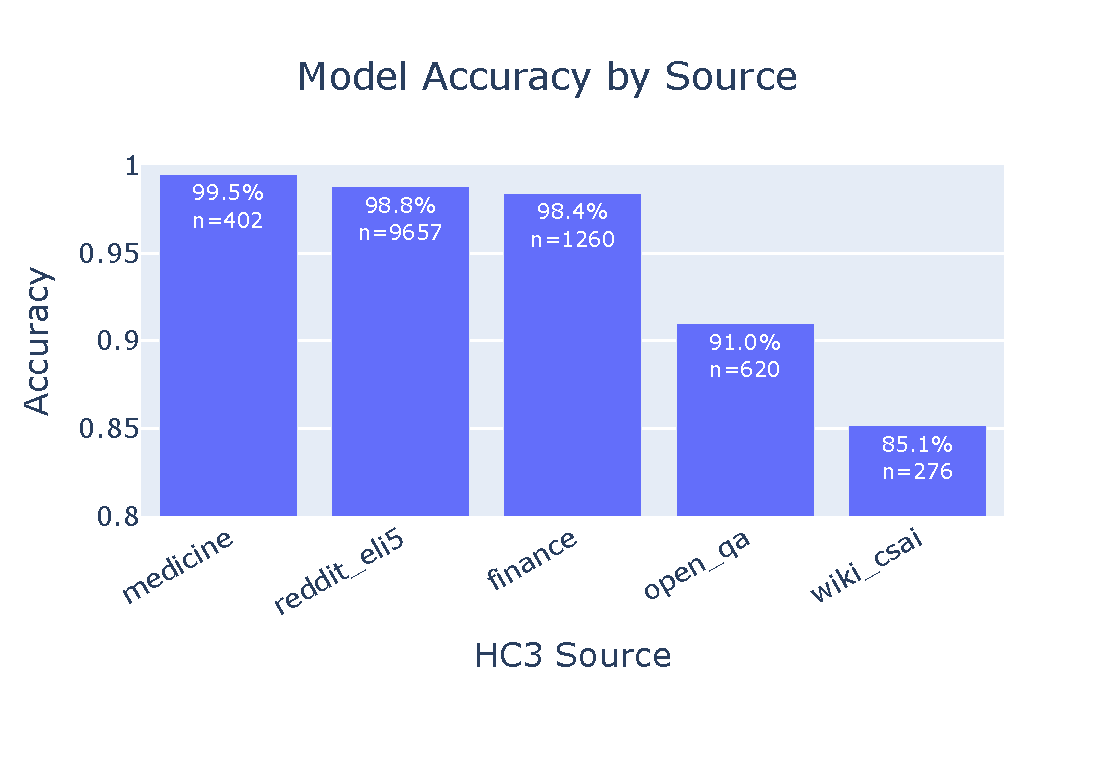
\includegraphics[width=\linewidth]{../train_outputs/figures/accuracy_by_source.pdf}
\caption{\large High accuracy across domains shows strong generalization.}
\end{figure}
\end{block}

\end{column}

\separatorcolumn

% ==================== COLUMN 2 ====================
\begin{column}{\colwidth}

\begin{block}{Methodology}

\textbf{Dataset:}
\vspace{-0.4em}
\begin{itemize}
\item HC3 (Human vs ChatGPT)
\item Multiple domains (Reddit, StackExchange)
\end{itemize}

\textbf{Model:}
\vspace{-0.4em}
\begin{itemize}
\item TF-IDF features
\item Logistic Regression
\item Interpretable coefficients
\end{itemize}

\textbf{Evaluation:}
\vspace{-0.4em}
\begin{itemize}
\item Accuracy
\item Source generalization
\end{itemize}

\end{block}

\vspace{-0.3cm}

\begin{block}{Model Confidence Distribution}
\begin{figure}
\centering
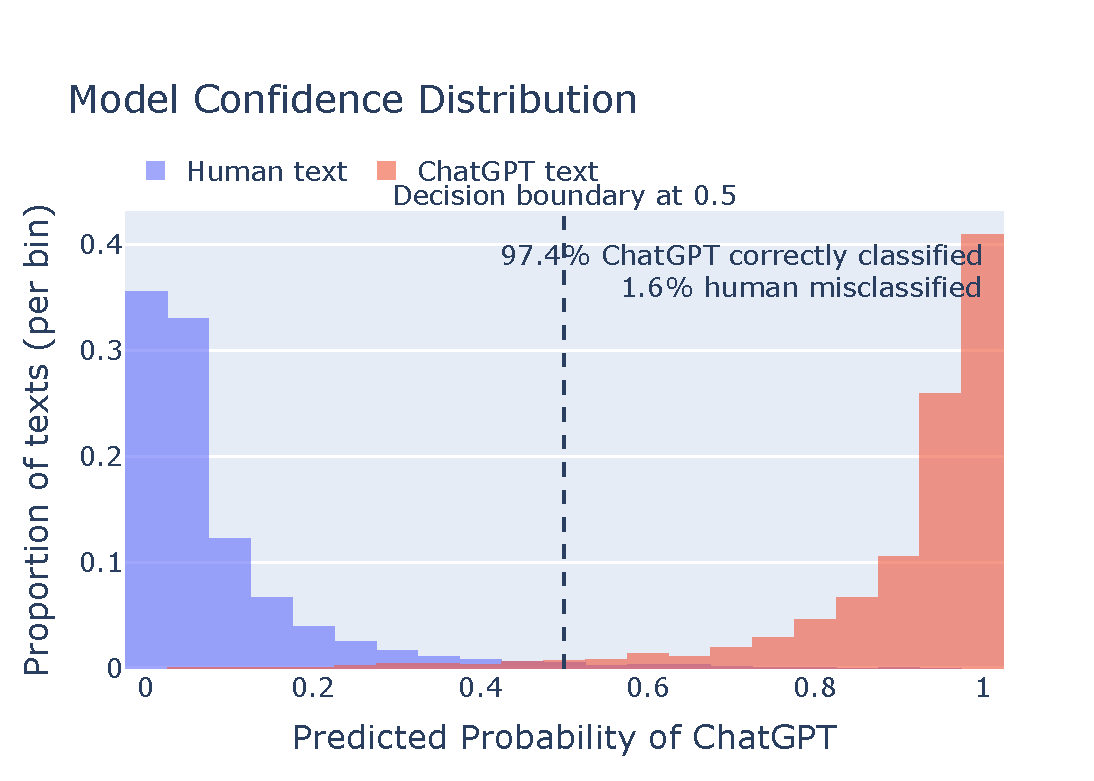
\includegraphics[width=\linewidth]{../train_outputs/figures/score_distribution.pdf}
\caption{\large Strong separation between human and AI predictions.}
\end{figure}
\end{block}

\end{column}

\separatorcolumn

% ==================== COLUMN 3 ====================
\begin{column}{\colwidth}

\begin{block}{Feature Importance}
\begin{figure}
\centering
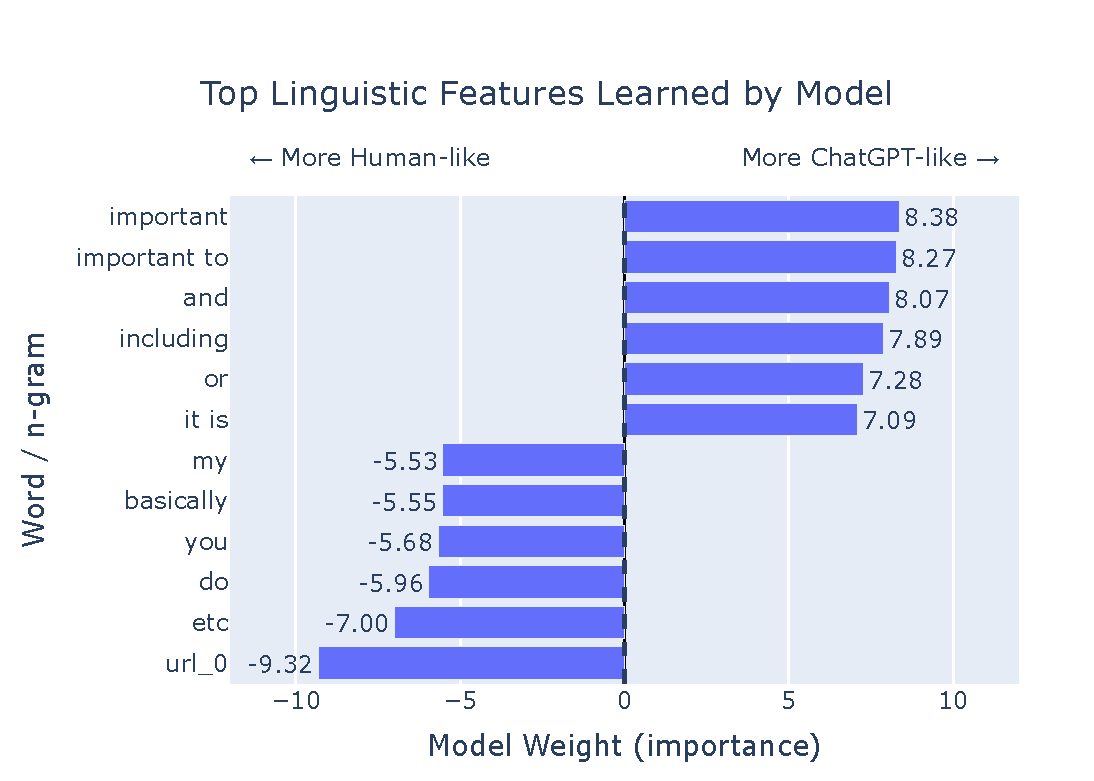
\includegraphics[width=\linewidth]{../train_outputs/figures/feature_importance.pdf}
\caption{\large Linguistic features distinguishing AI vs human writing.}
\end{figure}
\end{block}

\vspace{-0.3cm}

\begin{block}{Findings}

\textbf{Observations:}
\begin{itemize}
\item AI text is more stylistically consistent
\item Specific phrases strongly indicate LLM output
\item Human text is more varied
\end{itemize}

\textbf{Implications:}
\begin{itemize}
\item Lightweight models are highly effective
\item Interpretability provides clear insight
\item Detection may become harder as models improve
\end{itemize}

\end{block}

\end{column}

\separatorcolumn
\end{columns}
\end{frame}

\end{document}